%%%%%%%%%%%%%%%%%%%%%%%%%%%%%%%%%%%%%%%%%%%%%%%%%%%%%%%%%%%%
%%% ELIFE ARTICLE TEMPLATE
%%%%%%%%%%%%%%%%%%%%%%%%%%%%%%%%%%%%%%%%%%%%%%%%%%%%%%%%%%%%
%%% PREAMBLE 
\documentclass[9pt,lineno]{elife}
% Use the onehalfspacing option for 1.5 line spacing
% Use the doublespacing option for 2.0 line spacing
% Please note that these options may affect formatting.
% Additionally, the use of the \newcommand function should be limited.

\newcommand{\pKa}{p\textit{K}\textsubscript{a}}
\newcommand{\psKa}{p\textsubscript{s}\textit{K}\textsubscript{a}}
\newcommand{\logD}{log~\textit{D}}
\newcommand{\logP}{log~\textit{P}}

\usepackage{lipsum} % Required to insert dummy text
\usepackage[version=4]{mhchem}
\usepackage{siunitx}
\DeclareSIUnit\Molar{M}
\usepackage[colorinlistoftodos]{todonotes}
\usepackage{gensymb}
\usepackage{mhchem}
\usepackage{wrapfig}
\usepackage{booktabs}
\usepackage[flushleft]{threeparttable}


%%%%%%%%%%%%%%%%%%%%%%%%%%%%%%%%%%%%%%%%%%%%%%%%%%%%%%%%%%%%
%%% ARTICLE SETUP
%%%%%%%%%%%%%%%%%%%%%%%%%%%%%%%%%%%%%%%%%%%%%%%%%%%%%%%%%%%%
\title{Overview of SAMPL6 small molecule \pKa{} prediction challenge}

\author[1,2]{Mehtap Işık}
\author[1,3]{Ari\"{e}n S. Rustenburg}
\author[1,4]{Andrea Rizzi}
\author[5]{Caitlin Bannan}
\author[6]{Marilyn Gunner}
\author[7]{David L. Mobley}
\author[1*]{John D. Chodera}

\affil[1]{Computational and Systems Biology Program, Sloan Kettering Institute, Memorial Sloan Kettering Cancer Center, New York, NY 10065, United States}
\affil[2]{Tri-Institutional PhD Program in Chemical Biology, Weill Cornell Graduate School of Medical Sciences, Cornell University, New York, NY 10065, United States}
\affil[3]{Graduate Program in Physiology, Biophysics, and Systems Biology, Weill Cornell Medical College, New York, NY 10065, United States}
\affil[5]{?}
\affil[6]{Department of Pharmaceutical Sciences and Department of Chemistry, University of California,
Irvine, Irvine, California 92697, United States}
\corr{john.chodera@choderalab.org}{JDC}

%%%%%%%%%%%%%%%%%%%%%%%%%%%%%%%%%%%%%%%%%%%%%%%%%%%%%%%%%%%%
%%% ARTICLE START
%%%%%%%%%%%%%%%%%%%%%%%%%%%%%%%%%%%%%%%%%%%%%%%%%%%%%%%%%%%%

\begin{document}

\maketitle

%%%%%%%%%%%%%%%%%%%%%%%%%%%%%%%%%%%%%%%%%%%%%%%%%%%%%%%%%%%%
% Abstract
%%%%%%%%%%%%%%%%%%%%%%%%%%%%%%%%%%%%%%%%%%%%%%%%%%%%%%%%%%%%
\begin{abstract}
\todo[inline]{Complete abstact.}
- number of submissions  

- summary of analysis  

- difficulties observed  

\end{abstract}
%%%%%%%%%%%%%%%%%%%%%%%%%%%%%%%%%%%%%%%%%%%%%%%%%%%%%%%%%%%%
% Keywords and Abbreviations
%%%%%%%%%%%%%%%%%%%%%%%%%%%%%%%%%%%%%%%%%%%%%%%%%%%%%%%%%%%%
\subsection{Keywords}
SAMPL $\cdot$ blind prediction $\cdot$ \pKa{} $\cdot$ small molecule $\cdot$ macroscopic \pKa $\cdot$ microscopic \pKa  $\cdot$ macroscopic protonation state $\cdot$ microscopic protonation state

\subsection{Abbreviations}
\begin{description}
\item[SAMPL] Statistical Assessment of the Modeling of Proteins and Ligands
\item[\pKa]  --${\log_{10}}$ acid dissociation equilibrium constant 
\item[SEM] Standard error of the mean
\end{description}
\todo[inline]{Complete abbreviations}

%%%%%%%%%%%%%%%%%%%%%%%%%%%%%%%%%%%%%%%%%%%%%%%%%%%%%%%%%%%%
% Introduction
%%%%%%%%%%%%%%%%%%%%%%%%%%%%%%%%%%%%%%%%%%%%%%%%%%%%%%%%%%%%
\section{Introduction}
\todo[inline]{Complete introduction section.}

\todo[inline]{Importance of small molecule pKa prediction for pharmaceutical efforts.}

\todo[inline]{Explain why we are doing a pKa challenge and connect to past and previous challenges}
SAMPL (Statistical Assessment of the Modeling of Proteins and Ligands). About SAMPL challenges: Collectively, these challenges have assessed the effects of force field accuracy, solvation models, pKa and tautomer predictions.  

During the SAMPL5 challenge, log D predictions experienced difficulties predicting log D values accurately, unless protonation states and tautomers were taken into account.

For this iteration of the SAMPL challenge, we have taken one step back and isolated just the problem of predicting solvent protonation states.

This is the first time a blind pKa prediction challenge has been fielded as part of SAMPL. 
In this first iteration of the challenge, we aimed to assess the performance of current pKa prediction methods and isolate potential causes of inaccurate pKa estimates, with the aim of determining how pKa prediction inaccuracies might impact predicted affinities for drug-like molecules. 
For example, for both logD and binding affinity predictions, any error in predicting the free energy of accessing a minor protonation state in solution that becomes dominant in the complex will directly add to the error in the predicted transfer or binding free energy. 

Challenge goal: determining how pKa prediction inaccuracies might impact predicted affinities for drug-like molecules. For example, for both logD and binding affinity predictions, any error in predicting the free energy of accessing a minor protonation state in solution that becomes dominant in the complex will directly add to the error in the predicted transfer or binding free energy. 

Reason for blind pKa challenge:
- Impact on binding affinity predictions
- Impact on logD predictions (SAMPL6)
- Drug-like molecules are especially challenging.




Protonation state effects were a dominant accuracy-limiting factor for logD from SAMPL5, and should also be accuracy-limiting in binding free energy predictions.
Errors is \pKa{} predictions can cause modeling the wrong charge, protonation and tautomerization states which affect hydrogen bonding opportunities and overall dipole moment of the ligand.

\todo[inline]{Explain the physics of the predicted property}
\todo[inline]{EQUATION: pKa equation}
\todo[inline]{EQUATION: free energy of protonation state equation}
\todo[inline]{Introducing linear protonation state free energy diagram}
\todo[inline]{FIGURE: linear plot of free energy vs pH }

\todo[inline]{FIGURE: a diagram illustrating the ways in which the pKa errors can influence prediction errors for binding affinities}


\todo[inline]{Overview of kinds of pKa prediction methods available  (ML, QM, empirical methods ... }

\todo[inline]{Explain challenge design.}

Experimental macroscopic pKa values were measured using a UV-metric assay performed using a Sirius T3 [cite exp. paper ]  supported by Merck, MRL,  Rahway NJ.  
\todo[inline]{Figure: }

\begin{figure}
\begin{center}
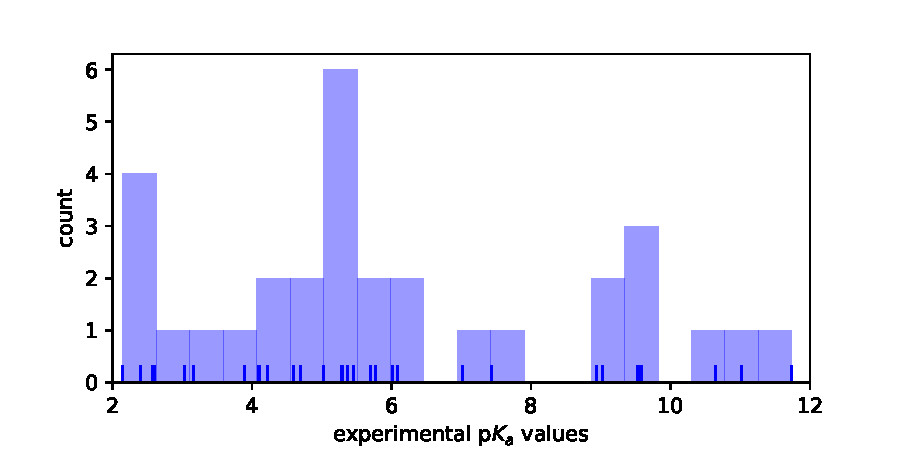
\includegraphics[width=0.65\linewidth]{figures/distribution_of_exp_pKas.pdf}
\caption{{\bf Distribution of experimental \pKa{} values of 24 compounds in SAMPL6 pKa challenge. } Spectrophotometric \pKa{} measurements were collected with Sirius T3. \todo[inline]{Add reference to pKa experiments manuscript.} Five compounds have multiple measured \pKa{}s in the range of 2-12.   
}
\label{fig:dist_exp_pKas}
\end{center}
\end{figure}

Communicate concepts behind challenge design and why we made specific choices:
Explain why we have types I, II, III
Explain why we preenumerated microstates

Participants had the option to submit predictions in one of 3 categories: Microscopic pKa values (type I), microscopic state populations (type II), or macroscopic pKa values (type III).

The comparison between macroscopic and microscopic pKa values is not always a straightforward one. 

Overview of available pKa prediction methods and methods that participated in SAMPL6. [Reminder to cite all papers here.]


\todo[inline]{Explain future direction for this challenge}
Challenge path: predict pKas, give people pKas to predict logDs on same molecules, then predict for new set of compounds logDs without provided pKas.
\todo[inline]{Explain potantial benefits of these challenge}
Improving computational methods...

%%%%%%%%%%%%%%%%%%%%%%%%%%%%%%%%%%%%%%%%%%%%%%%%%%%%%%%%%%%%
% Methods
%%%%%%%%%%%%%%%%%%%%%%%%%%%%%%%%%%%%%%%%%%%%%%%%%%%%%%%%%%%%
\section{Methods}

\subsection{Structure and logistics of the SAMPL6 pKa prediction challenge}
\todo[inline]{Describe the structure of SAMPL6 pKa challenge}
- When instructions and input files were made available

- Challenge dates

- Input files

- What to predict? Three type of submissions.

- Multiple submissions allowed

- Predicting the pKa values of the whole set wasn't a requirement. 

- 2nd D3R/SAMPL Workshop took place in La Jolla, San Diego on Feb 22-23, 2018.

\subsection{Analysis metrics for submission performance}
- Root mean squared error (RMSE)

- Mean absolute error (MAE)

- Mean Error (ME)

- Square of Pearson Correlation Coefficient (R\textsuperscript{2})

- Slope of prediction vs. experimental value linear fit

Uncertainty in each performance statistic was calculated by bootstapping (10,000) to estimate 95\% confidence intervals.

\subsection{Enumeration of requested prediction microscopic protonation states}
1. OpenEye (filter out resonance structures), Epik  

2. Participant supplied structures  

\subsection{Closest method for matching experimental and predicted pKas}
\todo[inline]{Explain closest method}

\subsection{Hungarian method for matching experimental and predicted pKas}
\todo[inline]{Explain Hungarian method}

\subsection{Matching experimental and predicted pKas based on microstate populations}
\todo[inline]{Figure out how to do this. Bas's network map will be useful.}

\subsection{Comparison of errors/performance against molecular descriptors} 
\todo[inline]{Look for correlation with descriptors, and potential explanation for errors. Keep spurious correlations in mind if we have many descriptors.}

%%%%%%%%%%%%%%%%%%%%%%%%%%%%%%%%%%%%%%%%%%%%%%%%%%%%%%%%%%%%
% Results
%%%%%%%%%%%%%%%%%%%%%%%%%%%%%%%%%%%%%%%%%%%%%%%%%%%%%%%%%%%%
\section{Results}

\subsection{Analysis of macroscopic \pKa{} predictions (Type III)}

\todo[inline]{A paragraph to explain the submission methods}
\todo[inline]{Null model 1: pKa prospector lookup}
\todo[inline]{Null model 2: ?}
\todo[inline]{TABLE: Error statistics for all participants}
\todo[inline]{FIGURE: Histograms of macrocopic pKa prediction statistics for all participants}
\todo[inline]{Check if top few performing methods are consistent between error metrics. }
\todo[inline]{FIGURE: Prediction vs experiment scatter plots for top 4-6 methods.)}
\todo[inline]{FIGURE: Violin plots of Delta pKa error to identify compounds that were frequently mispredicted (both closest/hungarian methods)}


\todo[inline]{Explain rationale behind how we analyze the data and determine success/failure}
\todo[inline]{Performance comparison of different methods, grouped by methods class}
\todo[inline]{Analysis of 4-aminoquinazoline series}

\todo[inline]{Assessment of individual methods by each of our analysis methods}

\todo[inline]{Assessment of the groups of methods}

\todo[inline]{Null model for macroscopic pKa predictions}


\subsection{Analysis of microscopic \pKa{} predictions (Type I \& II)}
\todo[inline]{FIGURE: Ranking of microscopic pKa prediction error for all participants}

\todo[inline]{FIGURE: Violin plots of Delta pKa error to identify compounds that were frequently mispredicted (both closest/hungarian methods)}

\todo[inline]{Assessment of individual methods by each of our analysis methods}

\todo[inline]{Assessment of the groups of methods}

\todo[inline]{Does type II predictions capture linear trend in DeltaG vs pH plot}

\todo[inline]{Calculation of predicted macroscopic pKas and comparison to experiment}
\todo[inline]{Performance comparison of different methods, grouped by methods class}
\todo[inline]{Comparison of predicted microstates using consensus set of transitions of high accuracy prediction methods} the consensus of predictions might give some indication here too of whether we're dealing with mono or polyprotic compounds

\todo[inline]{Analysis of 4-aminoquinazoline series}

\todo[inline]{How differently do different methods predict microscopic transitions? (method vs method correlation plot to see if methods predict the same microstate pairs or not)}


%%%%%%%%%%%%%%%%%%%%%%%%%%%%%%%%%%%%%%%%%%%%%%%%%%%%%%%%%%%%
% Discussion
%%%%%%%%%%%%%%%%%%%%%%%%%%%%%%%%%%%%%%%%%%%%%%%%%%%%%%%%%%%%
\section{Discussion}
\todo[inline]{Do any methods predict within experimental accuracy (how is the field doing overall)?}
\todo[inline]{Common challenging factors for accurate pKa predictions. Tautomers, Heterocycles etc.}

\subsection{Discussion of matching experimental and predicted values}
\todo[inline]{Difficulty of assessing predicted pKas using experimental data: matching problem}
\todo[inline]{Explain rationale behind how we analyze the data and determine success/failure}


\subsection{Prediction performance of individual molecules}
\todo[inline]{Which chemical structures make pKa predictions more difficult?}
SAMPL6 pKa set consisted of only 24 small molecules which limits our ability to do statistical analysis to determine which chemical substructures contribute to greater errors in pKa predictions.
\todo[inline]{Illustration/explanation of effects where microscopic pKas and macroscopic pKas can differ}

\todo[inline]{Are there any correlations between molecular descriptors and pKa errors?}

\todo[inline]{What can we learn from failures? Which physical effects are driving failures?}

\todo[inline]{How do accuracy limitations in small molecule pKa prediction translate into modeling errors in ligand affinity prediction?}


\subsection{Advice for future challenges}

\todo[inline]{Discuss what can be done to further improve future challenges}
How can we maximize what we learn?
What should we have people predict?
How should we select compounds / measure pKas?

\todo[inline]{Suggestions about challenge construction}

Enumeration of protonation states before predictions (which states does one need to consider?)

\todo[inline]{Suggestions about challenge analysis}

NMR experimental techniques could be used to validate microstate information in future challenges



%%%%%%%%%%%%%%%%%%%%%%%%%%%%%%%%%%%%%%%%%%%%%%%%%%%%%%%%%%%%
% Conclusion
%%%%%%%%%%%%%%%%%%%%%%%%%%%%%%%%%%%%%%%%%%%%%%%%%%%%%%%%%%%%
\section{Conclusion}


%%%%%%%%%%%%%%%%%%%%%%%%%%%%%%%%%%%%%%%%%%%%%%%%%%%%%%%%%%%%
% Code and Data Availability
%%%%%%%%%%%%%%%%%%%%%%%%%%%%%%%%%%%%%%%%%%%%%%%%%%%%%%%%%%%%
\section{Code and data availability}
\begin{minipage}{15cm}
\begin{itemize}

\item SAMPL6 \pKa{} challenge instructions, submissions, experimental data and analysis is available at  \href{https://github.com/MobleyLab/SAMPL6}{https://github.com/MobleyLab/SAMPL6}

\end{itemize}
\end{minipage}


%%%%%%%%%%%%%%%%%%%%%%%%%%%%%%%%%%%%%%%%%%%%%%%%%%%%%%%%%%%%
% Overview of supplementary information
%%%%%%%%%%%%%%%%%%%%%%%%%%%%%%%%%%%%%%%%%%%%%%%%%%%%%%%%%%%%
\section{Overview of supplementary information}

\paragraph{Organized in SI document:}

\begin{itemize}
\item TABLE SI 1: ???

\end{itemize}

\paragraph{Extra files:}  
\begin{itemize}
\item Any extra files
\end{itemize}


%%%%%%%%%%%%%%%%%%%%%%%%%%%%%%%%%%%%%%%%%%%%%%%%%%%%%%%%%%%%
% Author Contributions 
%%%%%%%%%%%%%%%%%%%%%%%%%%%%%%%%%%%%%%%%%%%%%%%%%%%%%%%%%%%%
\section{Author Contributions}

Conceptualization, MI, JDC, CB, DLM ; Methodology, MI, JDC ; Software, MI, AR, ASR ; Formal Analysis, MI, ASR, AR ; Investigation, MI ; Resources, JDC;  Data Curation, MI ; Writing-Original Draft, MI, JDC; Writing - Review and Editing, MI, ASR, AR, CB, DLM, JDC; Visualization, MI, AR ; Supervision, JDC, DLM, CB, ASR ; Project Administration, MI ; Funding Acquisition, JDC, DLM.

%(Follow the \href{http://www.cell.com/pb/assets/raw/shared/guidelines/CRediT-taxonomy.pdf}{CRediT Taxonomy})

%%%%%%%%%%%%%%%%%%%%%%%%%%%%%%%%%%%%%%%%%%%%%%%%%%%%%%%%%%%%
% Acknowledgments 
%%%%%%%%%%%%%%%%%%%%%%%%%%%%%%%%%%%%%%%%%%%%%%%%%%%%%%%%%%%%
\section{Acknowledgments}

\todo[inline]{Complete acknowledgments section.}
MI, ASR, and JDC acknowledge support from the Sloan Kettering Institute.
JDC acknowledges support from NIH grant P30 CA008748. 
MI acknowledges Doris J.\ Hutchinson Fellowship. 
We thank Brad Sherborne for his valuable insights at the conception of the \pKa{} challenge and connecting us with Timothy Rhodes and Dorothy Levorse who were able to provide resources and expertise for experimental measurements performed at MRL. 
We acknowledge Paul Czodrowski who provided feedback on multiple stages of this work: challenge construction, purchasable compound selection and manuscript. 
MI, ASR, AR and JDC are grateful to OpenEye Scientific for providing a free academic software license for use in this work.

Mike Chui
%\todo[inline]{JDC: Can we cite the ORCIDs of people we thank in this work?}

%%%%%%%%%%%%%%%%%%%%%%%%%%%%%%%%%%%%%%%%%%%%%%%%%%%%%%%%%%%%
% Disclosures 
%%%%%%%%%%%%%%%%%%%%%%%%%%%%%%%%%%%%%%%%%%%%%%%%%%%%%%%%%%%%
\section{Disclosures}

JDC is a member of the Scientific Advisory Board for Schr\"{o}dinger, LLC.
DLM is a member of the Scientific Advisory Board of OpenEye Scientific Software.

%\nocite{*} % This command displays all refs in the bib file. PLEASE DELETE IT BEFORE YOU SUBMIT YOUR MANUSCRIPT!
\bibliography{elife-sample,sampl}

%%%%%%%%%%%%%%%%%%%%%%%%%%%%%%%%%%%%%%%%%%%%%%%%%%%%%%%%%%%%
% Supplementary Information
%%%%%%%%%%%%%%%%%%%%%%%%%%%%%%%%%%%%%%%%%%%%%%%%%%%%%%%%%%%%
%\newpage
%\section{Supplementary Information}






\end{document}
